\documentclass[12pt,a4paper]{report}
\begin{comment}
\usepackage{amsmath,amsthm,amssymb,mathrsfs,graphicx,comment,blindtext,subfiles,tikz}
\usepackage[noend]{algorithmic} %algorithmic environment
\usetikzlibrary{shapes.geometric,calc}
\allowdisplaybreaks


\newtheorem{theorem}{Theorem}[section]
\newtheorem{definition}[theorem]{Definition}
\newtheorem{example}[theorem]{Example}
\newtheorem{corollary}[theorem]{Corollary}
\newtheorem{lemma}[theorem]{Lemma}
\newtheorem{proposition}[theorem]{Proposition}
\newtheorem{remark}[theorem]{Remark}
\newtheorem{algorithm}[theorem]{Algorithm}

\renewcommand{\baselinestretch}{1.5}
\renewcommand{\algorithmicrequire}{\textbf{Input:}}
\renewcommand{\algorithmicensure}{\textbf{Output:}}

%% Replace init/inif with \initial or "in"
\DeclareMathOperator{\initial}{in}
\end{comment}
\begin{document}

\chapter{Tracking Groebner Walk Progress}
Most of the implementations of the Groebner Walk in various Computer Algebra Systems (CAS) do not have any sort of tracking, in the form of progress or status bars, of the Groebner Walk. This means that, after initiating computation but before the algorithm terminates, there is no indication of the remaining distance that the Groebner Walk needs to traverse, as well as any estimation of how long the remaining distance will take to traverse. This is especially frustrating given the difficulty and computational complexity of Groebner Bases in general, especially those that encode much more information within them e.g. Bases with lexicographical ordering.

Again, like the Groebner Walk algorithm itself, there does not exist one right way to implement this. However, we would like our tracking progress algorithm to satisfy a few basic functionalities:

\begin{definition}
Define a distance function $d : \mathbb R^{n} \times \mathbb R^{n} \rightarrow \mathbb R_{\geq 0}^{n}$. For points $x, y , z \in \mathbb R^{n}$:

\begin{enumerate}
    \item $d(x,y) = 0 \Longleftrightarrow x = y$
    \item $d(x,y) = d(y,x)$
    \item $d(x,y) \leq d(x,z) + d(z,y)$
\end{enumerate}
\end{definition}

This merely is the definition of the metric and this can be used as a reference to compare potential distance measuring functions to, since any function that satisfies the above definition with have the required properties. 

Alternatively, we could rephrase this definition from conditions we want our distance function to satisfy into types of failure, conditions we want our function to avoid instead.

\begin{definition}
Define a distance function $d : \mathbb R^{n} \times \mathbb R^{n} \rightarrow \mathbb R_{{\geq 0}^{n}}$.  Let $x, y, z \in \mathbb R_{n}$.

\begin{enumerate}
    \item Failure state 1 (distance increases): $d(x,y) < d(x,z) + d(z,y)$ 
    \item Failure state 2 (infinitesimal steps): Distance progressed between successive steps is infinitesimally small.
    \item Failure state 3 (computational bottleneck):  Time spent running the distance function becomes too large or even the bottleneck in the whole computation.
    \item Failure state 4 (Positive distance endpoint): Algorithm terminates when distance function has value $\geq 0$.
\end{enumerate}
\end{definition}

Now we have defined what we want our distance function to avoid, we can then attempt to define some distance function and check that it does not have one or more of these failure states.

\section{Facet Oriented Methods}

\subsection{Barycentric Method}
To begin, we could explain a very simple method of measuring distance. It is done in the following fashion:

\begin{enumerate}
    \item Treat each cone $C_{\prec} (I)$ we enter as a single point $c$, that point being the barycentre of the cone.
    \item Distance is measured in a straight line, from the current cones' barycentre $C_{\prec_{1}} (I)$  to the target cones' barycentre $C_{\prec_{2}} (I)$.
\end{enumerate}
The simplest way of measuring this distance would be working in the Euclidean metric.

Hence, we can define the barycentres in coordinate form. Define the current cone barycentre as $c_{cur} = (a_{1}, \cdots, a_{n})$, and the target cone barycentre as $c_{tar} = (b_{1}, \cdots b_{n})$. Then, we can measure the total distance of the line $l$ between $c_{cur}$ and $c_{tar}$ in the following way:
\begin{equation*}
    dist(l) = \sqrt{\sum_{i=1}^{n} (a_{i} - b_{i})^{2}}
\end{equation*}

As we move through into a new cone, the barycentre of the new cone becomes the new $c_{cur}$.

%%Create Algorithm
\begin{algorithm}[Barycentric Distance Function]\
 \begin{algorithmic}[1]
 \REQUIRE{Cones $C_{<_{1}}, C_{<_{2}}$ in our required Groebner fan.}
 \ENSURE{Distance measured from $c_{cur} \in C_{<_{1}}$ to $c_{tar} \in C_{<_{2}}$.}
 \STATE{Find barycentre $c_{cur}, c_{tar}$ from cones $C_{<_{1}}, C_{<_{2}}$ respectively.}
 \STATE{$dist(l) = \sqrt{\sum_{i=1}^{n} (a_{i} - b_{i})^{2}}$.}
 \RETURN{dist(l)}
 \end{algorithmic}
 \end{algorithm}

%%%%%%%%%%%%%%%%%%%%%%Good Barycentre
\begin{figure}
\includegraphics[scale=0.5]{Chapters/images/Barycentre1.png}
\caption{An example of the Barycentric method}
\label{GoodBarycentre}
\end{figure}
%%%%%%%%%%%%%%%%%%%%%%%%%%%%%%%%%%%%%%%%

In \ref{GoodBarycentre}, we start with $C_{1}$ being the current cone, $c_{cur}$ being the current barycentre and $C_{4}$ being the target cone, $c_{tar}$ being the target barycentre. The distance at this step is measured by the distance of dashed line $l_{1}$. Following on, when the walk moves into $C_{2}$, then $c_{2}$ becomes the new $c_{cur}$, and so our distance at this step is dashed line $l_{2}$. We repeat this same process for $C_{3}$ and barycentre $c_{3}$.

However, this method is included for the sake of showing that finding a good distance function is a non-trivial task rather than being something we would seriously consider using. This method is simple to come up with, but fails on several counts. Firstly, it is not hard to demonstrate that distance could easily increase when measuring in this fashion. All that is needed is a walk whose line intersects a long thin cone near the apex of said cone. This means the barycentre is a significant distance away from the line and so is a poor choice to use for distance in this case. Secondly, calculating the barycentre involves finding all the edges of a particular cone and involves more calculations than we would like for this distance function. 

%%%%%%%%%%%%%%%%%%%%%%Bad Barycentre
\begin{figure}
\includegraphics[scale=0.5]{Chapters/images/Barycentre2.png}
\caption{A weakness of the Barycentric method}
\label{BadBarycentre}
\end{figure}
%%%%%%%%%%%%%%%%%%%%%%%%%%%%%%%%%%%%%%%%

Here, in this example, we can see visually that distance of $l_{2}$ is larger of $l_{1}$ despite the fact that cone $C_{2}$ is closer to the target cone than $C_{1}$. This implies that the distance, when walking from cone $C_{1}$, to $C_{2}$ and then $C_{3}$, that instead of having distance decrease monotonically, it instead increases. In this case, the barycentre $c_{2}$ is not representative of the cone as a whole. 

\subsection{Interior Point Method}
This is a weaker version of the Barycentric Method explored above, replacing calculating the barycentre of a cone with any interior point in a cone. This makes the distance function much easier to calculate, since determining if $p \in C_{\prec} (I)$, where $p$ is a point, can easily be done by checking if it satisfies the inequalities that make up the cone, rather than having to calculated all the edges of the cone. 

It still suffers from the increasing distance problem however, and this can be easily shown without any calculation directly from the Barycentric method. Refer back to \ref{BadBarycentre} and we can see visually that any interior point $p$ sufficiently distant from target cone $C_{3}$, such as the barycentre of cone $C_{2}$, would cause the same distance increasing problem as in the Barycentric method. 


\begin{algorithm}[Interior Point Distance Function]\
 \begin{algorithmic}[1]
 \REQUIRE{Cones $C_{<_{1}}, C_{<_{2}}$ in our required Groebner fan.}
 \ENSURE{Distance $d$ measured from $p_{1} \in C_{<_{1}}$ to $p_{2} \in C_{<_{2}}$.}
 \STATE{Randomly pick points $p_{1}, p_{2}$ in cones $C_{<_{1}}, C_{<_{2}}$ respectively.}
 \STATE{dist(l) = $\sqrt{\sum_{i=1}^{n} (a_{i} - b_{i})^{2}}$.}
 \RETURN{dist(l)}
 \end{algorithmic}
 \end{algorithm}

\subsection{L1 Ball Method}
We will use projection of L1 ball/unit circle ($|x| + |y| = 1)$, intersected with the positive orthant.

%%Is this necessary?
We will determine our straight line to use to calculate distance in the following way. From our starting cone $C_{\prec_{1}} (I)$ we draw a straight line to cone $C_{\prec_{2}} (I)$. When we enter a cone, there are two cases we need to consider. If the face of the new cone $C_{\prec} (I)$ that the line intersects is the closest to $C_{\prec_{2}} (I)$, we continue using this line. However, if there is a closer face we can use that the line does not intersect, we will redraw the straight line to $C_{\prec_{2}} (I)$ from cone $C_{\prec} (I)$ using this new face.

%%Reword this entire section
To calculate this, we do the following:
\begin{itemize}
    \item Given two vectors on a simplex, calculate the distance of these vectors.
    \item Normalise the vectors by dividing said vector by their respective distance.
    \item Distance between two points is the difference between normalised vectors, which is then normed. 
\end{itemize}

%%%%%%%%%%%%%%%%%%Norm with two points + distance image
\begin{figure}
\includegraphics[scale=0.4]{Chapters/images/L1Norm1.png}
\includegraphics[scale=0.6]{Chapters/images/L1Norm2.png}


\caption{Example of the L1 Norm method}
\end{figure}
%%%%%%%%%%%%%%%%%%%%%%%%%%%%%%%%%%%%%%%%

An example of this is 

%%Summarise into an algorithm
\begin{algorithm}[L1 Ball Distance Function]\
 \begin{algorithmic}[1]
 \REQUIRE{Cones $C_{<_{1}}, C_{<_{2}}$ in our required Groebner fan.}
 \ENSURE{Distance measured from $p_{1} \in C_{<_{1}}$ to $p_{2} \in C_{<_{2}}$.}
 \STATE{Randomly pick points $p_{1}, p_{2}$ in cones $C_{<_{1}}, C_{<_{2}}$ respectively.}
 \STATE{dist(l) = $\sqrt{\sum_{i=1}^{n} (a_{i} - b_{i})^{2}}$.}
 \RETURN{dist(l)}
 \end{algorithmic}
 \end{algorithm}

\subsection{Great Circle Distance Method}
 The Great Circle Distance, which is the distance between two points on the surface of a sphere, could be used as a measurement.
 
 This could be implemented, however the main formula used to measure this, the spherical law of cosines, can have large rounding errors due to the fact that, for $x \approx 0, cos(x) \approx 1$ (e.g. $cos(0.0001) = 0.9999999950...$

This makes this unsuitable as we would like to avoid this numerical instability.

\section{Line Oriented Methods}
\subsection{Hyperbola Method}
For this method, we can characterise the current and target point using a hyperbola on the positive orthant.

We can do this in the following way:

\begin{itemize}
    \item Draw a (rectangular) hyperbola, defined by $h = \prod_{x=1}^{n} x_{i} = 1$ in $\mathbb R^{n}$ for variables $x_{1}, \cdots, x_{n}$. For example, in $\mathbb{R^2}$, we have variables $x,y$, so our hyperbola is $xy = 1$.
    \item For a point $v_{j}$, draw a line passing through $v_{j}$ and origin O.
    \item Find the point of intersection between said line and the parabola, denote this as $v'_{i}$.
    \item Repeat process for other points $v_{k}$, to find intersections $v'_{k}$.
\end{itemize}


Ideally, we would like to measure the distance between $v'_{j}$ and $v'_{k}$ using the arc length, however there is no closed form expression to calculate this . Instead of attempting to work with or approximate the arc length, we will take the Euclidean distance between points $v'_{j}$ and $v'_{k}$ instead.

\begin{figure}
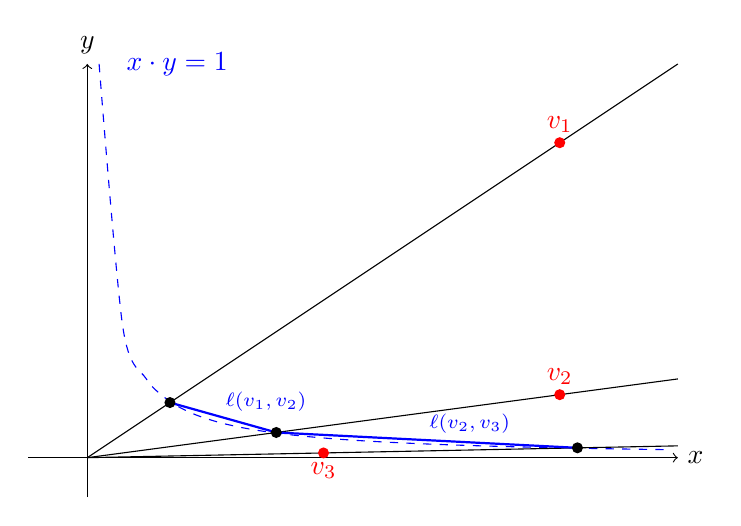
\begin{tikzpicture}[x=1.5cm,y=1cm]
  \draw[->] (-0.5, 0) -- (5, 0) node[right] {$x$};
  \draw[->] (0, -0.5) -- (0, 5) node[above] {$y$};
  \draw[dashed,yscale=0.5, domain=0.1:4.9, smooth, variable=\x, blue] plot ({\x}, {1/\x});
  \node[blue,anchor=west] at (0.25,5) {$x\cdot y=1$};
  \draw[] (0,0) -- (5,5);
  \draw[] (0,0) -- (5,1);
  \draw[] (0,0) -- (5,0.15);
  \coordinate (i1) at (0.7,0.7);
  \coordinate (i2) at (1.6,0.32);
  \coordinate (i3) at (4.15,0.125);
  \coordinate (v1) at (4,4);
  \coordinate (v2) at (4,0.8);
  \coordinate (v3) at (2,0.06);
  \draw[blue,thick] (i1) -- node[anchor=south west,xshift=-1mm,yshift=-0.5mm,font=\scriptsize] {$\ell(v_1,v_2)$} (i2) -- node[anchor=south west,xshift=-1mm,yshift=-0.5mm,font=\scriptsize] {$\ell(v_2,v_3)$} (i3);
  \fill (i1) circle (2pt);
  \fill (i2) circle (2pt);
  \fill (i3) circle (2pt);
  \fill[red] (v1) circle (2pt);
  \fill[red] (v2) circle (2pt);
  \fill[red] (v3) circle (2pt);
  \node[red,above] at (v1) {$v_1$};
  \node[red,above] at (v2) {$v_2$};
  \node[red,below] at (v3) {$v_3$};
  % \draw[scale=0.5, domain=-3:3, smooth, variable=\y, red]  plot ({\y*\y}, {\y});
\end{tikzpicture}
\caption{Example with points $v_{1}, v_{2}$ and $v_{3}$}
\end{figure}

In this example, for each point $v_{1}, v_{2}, v_{3}$, they can be represented on the hyperbola and then the distance between these points can be measured using the method we outlined earlier. Note that the distance from $v_{1}$ to $v_{2}$ is, visually, larger than $v_{2}$ to $v_{3}$. However, when measured using the hyperbola, it is clear that the distance of $l(v_{1}, v_{2})$ is smaller than distance of $l(v_{2}, v_{3})$.

There is a significant problem with using this to measure distance however, due to the fact that lexicographic ordering is represented by $\smash[b]{(1,\! \underbrace{0, 0,\cdots 0)\,}_\text{$n-1$ times}} \in \mathbb R^{n}$ in vector form.


This does not lie on the hyperbola, and so we cannot use the method of measuring distance for the last step. This means that when this method is used to measure distance in a Groebner walk that walks from some term ordering to the lexicographic ordering, the end point will be unknown.

\begin{algorithm}[Hyperbola Distance Function]\
 \begin{algorithmic}[1]
 \REQUIRE{Points  $p_{1} \in C_{<_{1}}$, $p_{2} \in C_{<_{2}}$.}
 \ENSURE{Distance measured from $p_{1} \in C_{<_{1}}$ to $p_{2} \in C_{<_{2}}$.}
 \STATE{Draw a hyperbola $\prod_{x=1}^{n} x_{i} = 1$ in $\mathbb R^{n}$ for variables $x_{1}, \cdots, x_{n}$.}
 \STATE{For points $v_{1}, \cdots, v_{k}$, draw lines passing through each point and origin O.}
 \STATE{Find the intersections of the lines $v'_{1}, \cdots, v'_{k}$.}
 \STATE{Distance between points $v'_{1}$ and $v'_{2}$ is the Euclidean distance measured by the line between them.}
 \RETURN{dist(l)}
 \end{algorithmic}
 \end{algorithm}

\subsection{Shifted Hyperbola Method}
Recalling the problems with the Hyperbola method (namely the lexicographic ordering not lying on the hyperbola), we can try to fix this by projecting onto a shifted hyperbola rather than the hyperbola used above ( $\prod_{x=1}^{n} x_{i} = 1$ ).

This can be done in the following way:
\begin{definition}
For vectors $v, w \in \mathbb R^{n}$, dummy variable $t$, constant $S \in \mathbb R_{\geq 0}$ denoting the shift and $cond_{v} = 1, cond_{w} = 1$:

\begin{equation*}
cond_{v} = cond_{v} \cdot (t \cdot v_{i} - \frac{1}{S}), cond_{w} = cond_{w} \cdot (t \cdot v_{i} - \frac{1}{S})
\end{equation*}

We repeat this for every element in vectors $v, w$ and then finally subtract $1$ from the final result. We then solve the polynomial and use the first non-imaginary root. This new parabola can then be used rather than the original parabola.
\end{definition}



A suitable shifting does solve the problem, but this simultaneously introduces another potential failstate (infintesimal steps) to the distance function, and so it seems that there is a tradeoff required.

These infintesimal steps occur due to this shifted projection. For example, take a list of vectors $(1,1), (2,1), (3,1), \cdots, (D,1) \in \mathbb R^{n}$, where $D \in \mathbb R $,  $D$ arbitrarily large. When these get projected onto the hyperbola, we have the following:
\begin{equation*}
\begin{split}
    & (1,1) \mapsto (1,1) \\ & (2,1) \mapsto (1,1) \\ & (3,1) \mapsto (1,1) \\  \cdots & \\ & (D,1) \mapsto (1,1)
\end{split}
\end{equation*}

Imagine that the list of vectors is the vector of each step of the Groebner Walk. The left hand side implies that there is a definitive change at each step and so progress is being made. However, when it is projected, all of them would be projected to the same vector, implying no progress is being made.

\chapter{Conclusion}

Over the course of this paper, we revisited several Groebner Walks , attempted to find appropriate distance functions for said Groebner Walks and implemented them into Singular. We have found that the Facet Oriented Walk is an infeasible variation on the Groebner Walk (unless the complexity of calculating all the edges of a facet reduces significantly). We have also found that implementing a distance function for Groebner Walks is far more difficult than initially expected and that there are far more potential failure states than first expected, especially given the seemingly intractable problems introduced by the Hyperbola/Shifted Hyperbola methods. Potential future improvements would be to continue to search for a satisfactory distance function for Straight Line Methods, as well as continuing to find new potential Groebner Walk methods as well as optimise currently existing ones.

\end{document}